\beamertemplateshadingbackground{white}{white}
\section{Stručný opis}
\begin{snimka}
 \frametitle{Elektronický kompas - Stručný opis}
   \begin{columns}[c]
   \only<1>
   {
    \begin{column}{0.6\textwidth}
     \begin{center}
        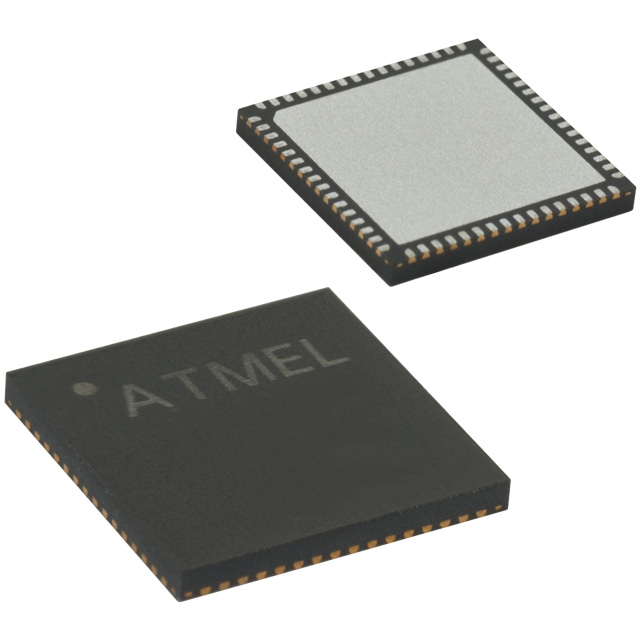
\includegraphics[width=0.8\textwidth]{obr/am7.jpg}
      \end{center}
    \end{column}
    }
   \only<2>
   {
    \begin{column}{0.6\textwidth}
     \begin{center}
        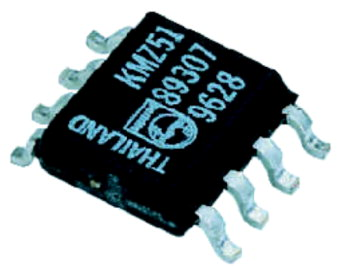
\includegraphics[width=0.8\textwidth]{obr/kmz.jpg}
      \end{center}
    \end{column}
    }

   \only<3>
   {
    \begin{column}{0.6\textwidth}
     \begin{center}
        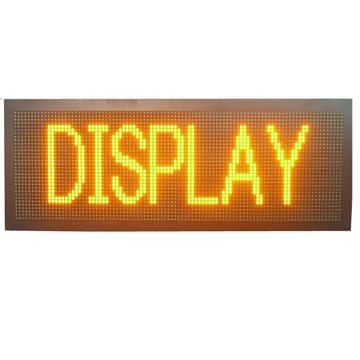
\includegraphics[width=0.8\textwidth]{obr/zobr.jpg}
      \end{center}
    \end{column}
    }

   \only<4>
   {
    \begin{column}{0.6\textwidth}
     \begin{center}
        
\includegraphics[width=0.8\textwidth]{obr/source.jpg}
      \end{center}
    \end{column}
    }

    \begin{column}{0.4\textwidth}
    \begin{block}{Stručný opis}
    \begin{enumerate}
         \item <+-| alert@+> Výber vhodného MCU.
         \item <+-| alert@+> Senzor, magnetický kompas
         \item <+-| alert@+> Zobrazovanie a vyhodnotovanie výsledkov
         \item <+-| alert@+> Kalibrácia pomocou sw
    \end{enumerate}
  \end{block}
        \end{column}
  \end{columns}
\end{snimka}